% !TEX TS-program = pdflatex
% !TEX encoding = UTF-8 Unicode

% This is a simple template for a LaTeX document using the "article" class.
% See "book", "report", "letter" for other types of document.

\documentclass[11pt]{article} % use larger type; default would be 10pt

\usepackage[utf8]{inputenc} % set input encoding (not needed with XeLaTeX)

%%% Examples of Article customizations
% These packages are optional, depending whether you want the features they provide.
% See the LaTeX Companion or other references for full information.

%%% PAGE DIMENSIONS
\usepackage{geometry} % to change the page dimensions
\geometry{a4paper} % or letterpaper (US) or a5paper or....
\geometry{margin=1in} % for example, change the margins to 2 inches all round
% \geometry{landscape} % set up the page for landscape
%   read geometry.pdf for detailed page layout information

\usepackage{graphicx} % support the \includegraphics command and options

% \usepackage[parfill]{parskip} % Activate to begin paragraphs with an empty line rather than an indent
\usepackage{amssymb}
\usepackage{amsmath}
%%% PACKAGES
\usepackage{booktabs} % for much better looking tables
\usepackage{array} % for better arrays (eg matrices) in maths
\usepackage{paralist} % very flexible & customisable lists (eg. enumerate/itemize, etc.)
\usepackage{verbatim} % adds environment for commenting out blocks of text & for better verbatim
\usepackage{subfig} % make it possible to include more than one captioned figure/table in a single float
% These packages are all incorporated in the memoir class to one degree or another...

%%% HEADERS & FOOTERS
\usepackage{fancyhdr} % This should be set AFTER setting up the page geometry
\pagestyle{fancy} % options: empty , plain , fancy
\renewcommand{\headrulewidth}{0pt} % customise the layout...
\lhead{}\chead{}\rhead{}
\lfoot{}\cfoot{\thepage}\rfoot{}

%%% SECTION TITLE APPEARANCE
\usepackage{sectsty}
\allsectionsfont{\sffamily\mdseries\upshape} % (See the fntguide.pdf for font help)
% (This matches ConTeXt defaults)

%%% ToC (table of contents) APPEARANCE
\usepackage[nottoc,notlof,notlot]{tocbibind} % Put the bibliography in the ToC
\usepackage[titles,subfigure]{tocloft} % Alter the style of the Table of Contents
\usepackage{bbm}
\usepackage{endnotes}

\renewcommand{\cftsecfont}{\rmfamily\mdseries\upshape}
\renewcommand{\cftsecpagefont}{\rmfamily\mdseries\upshape} % No bold!
\DeclareMathOperator*{\argmax}{arg\,max}
\DeclareMathOperator*{\argmin}{arg\,min}

\usepackage{graphicx}
\graphicspath{ {./pings/} }

\newcount\colveccount
\newcommand*\colvec[1]{
        \global\colveccount#1
        \begin{pmatrix}
        \colvecnext
}
\def\colvecnext#1{
        #1
        \global\advance\colveccount-1
        \ifnum\colveccount>0
                \\
                \expandafter\colvecnext
        \else
                \end{pmatrix}
        \fi
}

\newcommand{\norm}[1]{\left\lVert#1\right\rVert}

\title{Econometrics HW4}
\author{Michael B. Nattinger\footnote{I worked on this assignment with my study group: Alex von Hafften, Andrew Smith, and Ryan Mather. I have also discussed problem(s) with Emily Case, Sarah Bass, Katherine Kwok, and Danny Edgel.}}

\begin{document}
\maketitle

\section{Question 22.1}
\subsection{Part A}
Given the PDF of $e, \exists F(e)$, the corresponding CDF. Note now that $P(y_i \leq y | x_i = x) = P(x_i'\theta + e_i \leq y|x_i = x) = P(e_i\leq y-x_i'\theta|x_i = x).$ From the independence of $e,x$ we have: $P(e_i \leq y-x_i'\theta|x_i=x) = P(e_i \leq y-x_i'\theta) = F(y-x_i\theta).$ By differentiation we find $f(y|x) = f(f-x'\theta)$.
\subsection{Part B}
We have some functional form for the density of $e$ so we can write our objective function as (negative) log likelihood (negative since we are minimizing).  Then, $\rho_i(\theta) = - log(y_i - x_i\theta), \\ \psi_i(\theta) = \frac{\partial}{\partial \theta}\rho_i(\theta)  = \frac{f'(y_i - x_i'\theta)}{f(y_i - x_i'\theta)}x_i$.
\subsection{Part C}
$\Omega = E[\psi_i \psi_i'] = E[\left(\frac{f'(y_i - x_i'\theta)}{f(y_i - x_i'\theta)}\right)^2x_ix_i'] = E[\left(\frac{f'(e_i)}{f(e_i)}\right)^2x_ix_i'] = E[\left(\frac{f'(e_i)}{f(e_i)}\right)^2]E[x_ix_i']$. As stated in the textbook, for correctly specified MLE $Q=\Omega, V = \Omega^{-1} = E[\left(\frac{f'(e_i)}{f(e_i)}\right)^2]^{-1}E[x_ix_i']^{-1}$
\section{Question 23.1}
\subsection{Part A}
Due to the nonlinearity of $exp(\cdot )$, the conditional mean is nonlinear in $\theta$. This would be a nonlinear regression model.
\subsection{Part B}
We can define $\gamma = exp(\theta)$ and write $Y=\gamma + e$. Then we can estimate $\hat{\gamma} = \bar{Y}_n$, and obtain our estimate $\hat{\theta} = log(\gamma).$
\subsection{Part C}
M-estimators are invariant under reparameterization so this is the same.
\section{Question 23.2}
No. For even integer $\lambda$, $Y^{(\lambda)}$ is not invertible. Therefore one could not (uniquely) express $Y$ as a function of $X$ given parameters.
\section{Question 23.7}
We can calculate the SE as follows: $s=\sqrt{\frac{\partial m (x,\hat{\theta})}{\partial \theta} \hat{V} \frac{\partial m (x,\hat{\theta})}{\partial \theta'} }$. Then, \\$CI = [m(x,\hat{\theta})-1.96s,m(x,\hat{\theta})+1.96s]$ is an asymptotic $95\%$ confidence interval for $m(x).$
\section{Question 23.8} % stata

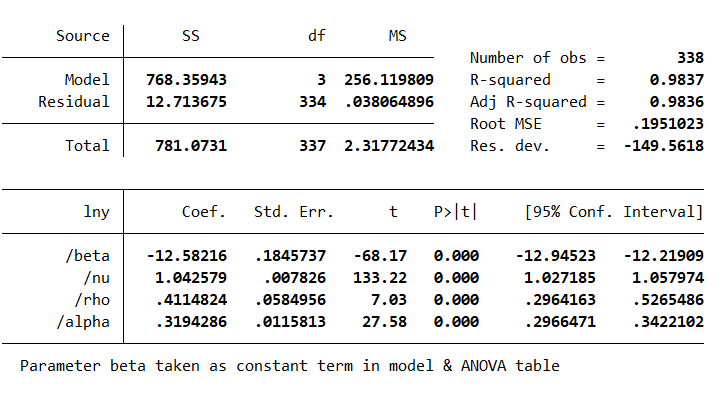
\includegraphics{p1}

$\hat{\sigma} = \frac{1}{1-\hat{\rho}} = 1.70.$ The estimated coefficients are almost all really close, but $\beta$ is not.

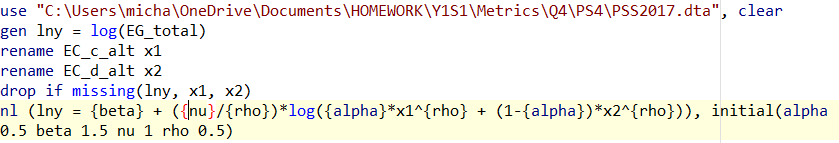
\includegraphics{p2}

\section{Question 24.3}
Fix $\tau$ and define $\theta$ as described in the problem. Note the following:
\begin{align*}
E[\psi(Y-\theta)] &= E[\tau - 1\{Y-\theta<0 \}]\\
 &= \tau - E[1\{Y<\theta \}]\\
&= \tau - P(Y<\theta)\\
&= 0\\
\Rightarrow P(Y<\theta) &= \tau,
\end{align*}
so $\theta$ is the $\tau$ quantile of $Y$.
\section{Question 24.4}
\subsection{Part A}
$E[Y|X] = E[X'\beta + e|X] = X'\beta + E[e|X] = X'\beta$ by the symmetry of the conditional distribution of $e$. Also by the conditional symmetry, $med[Y|X] = E[Y|X] = X'\beta$.
\subsection{Part B}
Asymptotically they are the same but under a finite sample they are different in general. This is because they minimize different criterion, and in general although the minimizers of squared error and absolute deviation will converge eventually there is no reason why they should be the same under a finite sample.
\subsection{Part C}
You would prefer LAD over OLS if you were worried about outliers in your data which may have too much of an influence in finite samples. Otherwise you would use OLS as it is conditionally unbiased and efficient in this context.
\section{Question 24.5}
Our colleague is being a bit ridiculous. The OLS estimate $\hat{\beta}_{ols}$ is guaranteed to have a lower $R^2$ than the LAD estimate $\hat{\beta}_{lad}$ by construction: \\\begin{align*}R^2_{ols} = 1 - \frac{(y-\hat{\beta}_{ols}x)'(y-\hat{\beta}_{ols}x)}{(y-\bar{y})'(y-\bar{y})} \geq  1 - \frac{(y-\hat{\beta}_{lad}x)'(y-\hat{\beta}_{lad}x)}{(y-\bar{y})'(y-\bar{y})} = R^2_{lad}.\end{align*} Comparing $R^2$ is an unfair test for determining which estimate to trust.
\section{Question 24.14} 

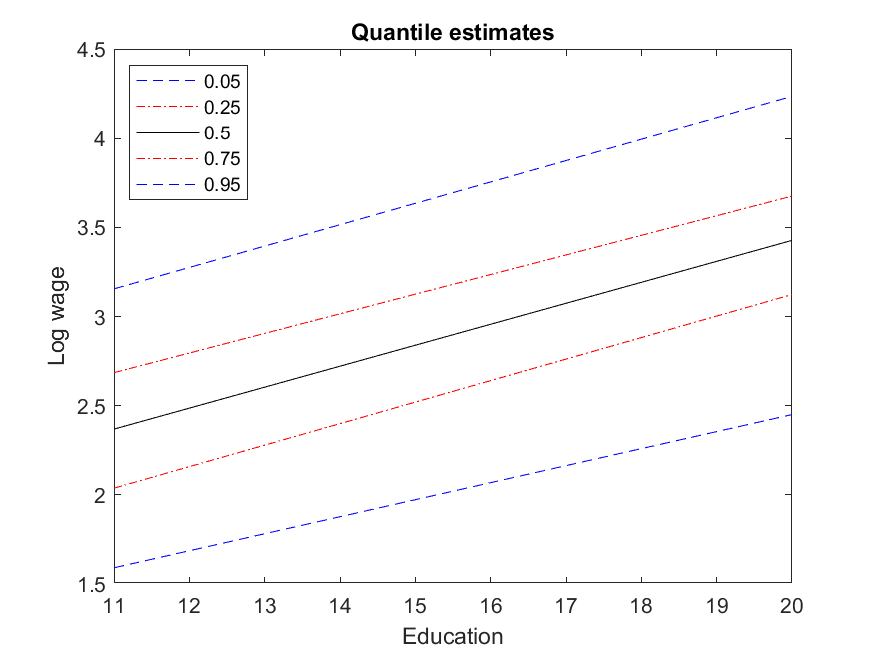
\includegraphics{qrfig}

The above figure shows the estimated quantiles of the conditional distributions of log wages, conditioning on education. The results indicate that the conditional distribution is approximately homoskedastic.

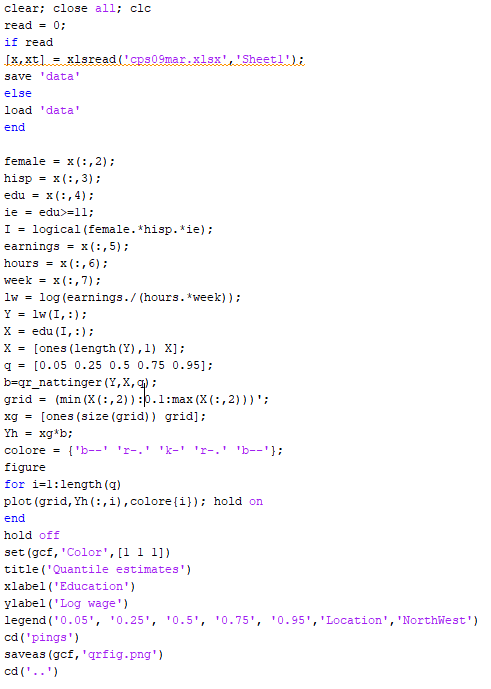
\includegraphics{p3}

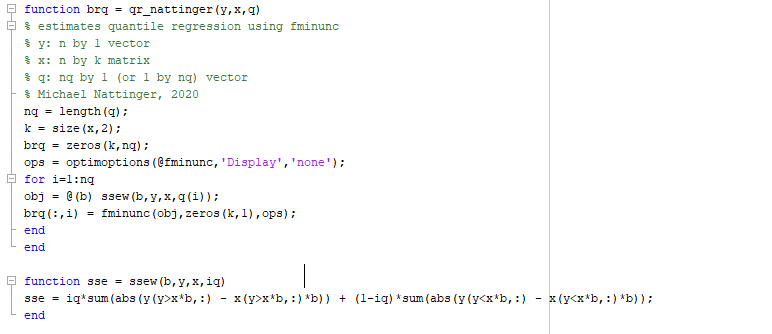
\includegraphics{p4}

\end{document}
